%%%%%%%%%%%%%%%%%%%%%%%%%%%%%%%%%%%%%%%%%%%%%%%%%%%%%%%%%%%%%%%%%%%%%%%%%%%%%%%%
% --- PREAMBLE --------------------------------------------------------------- %
%%%%%%%%%%%%%%%%%%%%%%%%%%%%%%%%%%%%%%%%%%%%%%%%%%%%%%%%%%%%%%%%%%%%%%%%%%%%%%%%

\documentclass[12pt, a4paper, twoside, openright]{report}
\usepackage{newtxtext}
\usepackage{textgreek}

\usepackage[margin=1in]{geometry}

\usepackage{amsmath}

\usepackage{minted}
\usepackage{mdframed}
\definecolor{bg}{rgb}{0.90,0.90,0.90}

\usepackage{subcaption}

\usepackage{authblk}

\usepackage[]{graphicx}
\usepackage{pgfplots}
\usepackage{pdfpages}
\usepackage[inkscapeformat=png]{svg}
\usepackage{circuitikz}
\usepackage{array}

%%%%%%%%%%%%%%%%%%%%%%%%%%%%%%%%%%%%%%%%%%%%%%%%%%%%%%%%%%%%%%%%%%%%%%%%%%%%%%%%
% --- FONT SIZES ------------------------------------------------------------- %
%%%%%%%%%%%%%%%%%%%%%%%%%%%%%%%%%%%%%%%%%%%%%%%%%%%%%%%%%%%%%%%%%%%%%%%%%%%%%%%%

\renewcommand   \footnotesize   {\fontsize{ 8pt}{ 9.6pt}\selectfont}
\renewcommand   \small          {\fontsize{10pt}{  12pt}\selectfont}
\renewcommand   \normalsize     {\fontsize{12pt}{14.4pt}\selectfont}
\renewcommand   \large          {\fontsize{14pt}{16.8pt}\selectfont}
\renewcommand   \Large          {\fontsize{16pt}{19.2pt}\selectfont}
\renewcommand   \LARGE          {\fontsize{18pt}{21.6pt}\selectfont}
\renewcommand   \huge           {\fontsize{20pt}{  24pt}\selectfont}
\renewcommand   \Huge           {\fontsize{22pt}{26.4pt}\selectfont}
\newcommand     \HUGE           {\fontsize{24pt}{28.8pt}\selectfont}

\newcommand     \sub            \textsubscript

%%%%%%%%%%%%%%%%%%%%%%%%%%%%%%%%%%%%%%%%%%%%%%%%%%%%%%%%%%%%%%%%%%%%%%%%%%%%%%%%
% --- PARAGRAPH SPACING ------------------------------------------------------ %
%%%%%%%%%%%%%%%%%%%%%%%%%%%%%%%%%%%%%%%%%%%%%%%%%%%%%%%%%%%%%%%%%%%%%%%%%%%%%%%%

%\edef\restoreparindent{\parindent=\the\parindent\relax}
%\usepackage[skip=\baselineskip]{parskip}
%\restoreparindent

%%%%%%%%%%%%%%%%%%%%%%%%%%%%%%%%%%%%%%%%%%%%%%%%%%%%%%%%%%%%%%%%%%%%%%%%%%%%%%%%
% --- TITLE FORMATTING ------------------------------------------------------- %
%%%%%%%%%%%%%%%%%%%%%%%%%%%%%%%%%%%%%%%%%%%%%%%%%%%%%%%%%%%%%%%%%%%%%%%%%%%%%%%%

\usepackage{titlesec}

\titleformat{\chapter}{
    \bf
    \huge
}{\thechapter}{1pt}{ }
\titlespacing{\chapter}{0pt}{2ex}{1ex}

\titleformat{\section}{
    \bf
    \LARGE
}{\thesection}{1pt}{ }

\titlespacing{\section}{0pt}{2ex}{1ex}

\titleformat{\subsection}{
    \bf
    \Large
}{\thesubsection}{1pt}{ }
\titlespacing{\subsection}{0pt}{2ex}{1ex}

\titleformat{\subsubsection}{
    \bf
    \large
}{\thesubsubsection}{1pt}{ }
\titlespacing{\subsubsection}{0pt}{2ex}{1ex}


%%%%%%%%%%%%%%%%%%%%%%%%%%%%%%%%%%%%%%%%%%%%%%%%%%%%%%%%%%%%%%%%%%%%%%%%%%%%%%%%
% --- ANNEX RELATED ---------------------------------------------------------- %
%%%%%%%%%%%%%%%%%%%%%%%%%%%%%%%%%%%%%%%%%%%%%%%%%%%%%%%%%%%%%%%%%%%%%%%%%%%%%%%%

\usepackage{acro}
\usepackage[
    sorting=none
]{biblatex}
\usepackage{hyperref}
\hypersetup{
    pdftitle=Documentation,
    colorlinks=true,
    linkcolor=black,
    filecolor=black,
    citecolor=black,
    urlcolor=cyan,
}
\usepackage[nottoc]{tocbibind}

\makeatletter
\newcommand{\emptypage}[1]{%
  \cleardoublepage
  \begingroup
  \let\ps@plain\ps@empty
  \pagestyle{empty}
  #1
  \cleardoublepage
  \endgroup
  }
\makeatletter


\DeclareAcronym{daw}{
    short=DAW,
    long=digital audio workstation
}

\DeclareAcronym{midi}{
    short=MIDI,
    long=musical instrument digital interface
}

\DeclareAcronym{pcb}{
    short=PCB,
    long=printed circuit board
}

\DeclareAcronym{opamp}{
    short=opamp,
    long=operational amplifier
}

\DeclareAcronym{usb}{
    short=USB,
    long=Universal Serial Bus
}

\DeclareAcronym{rms}{
    short=RMS,
    long=root mean square
}

\DeclareAcronym{eq}{
    short=EQ,
    long=equalizer
}

\DeclareAcronym{pa}{
    short=PA,
    long=Public Address,
    extra=System
}

\DeclareAcronym{pcm}{
    short=PCM,
    long=pulse code modulation
}

\DeclareAcronym{snr}{
    short=SNR,
    long=signal to noise ratio
}

\DeclareAcronym{dr}{
    short=DR,
    long=dynamic range
}

\DeclareAcronym{adc}{
    short=ADC,
    long=analog-to-digital converter
}

\DeclareAcronym{dac}{
    short=DAC,
    long=digital-to-analog converter
}

\DeclareAcronym{trs}{
    short=TRS,
    long=Tip-Ring-Sleeve,
    extra=a type of connector
}

\DeclareAcronym{ts}{
    short=TS,
    long=Tip-Sleeve,
    extra=a type of connector
}

\DeclareAcronym{rca}{
    short=RCA,
    long=Radio Corporation of America,
    extra=a type of connector
}


\DeclareAcronym{xlr}{
    short=XLR,
    long=External Line Return,
    extra=a type of connector
}









\addbibresource{cite.bib}

\begin{document}

%%%%%%%%%%%%%%%%%%%%%%%%%%%%%%%%%%%%%%%%%%%%%%%%%%%%%%%%%%%%%%%%%%%%%%%%%%%%%%%%
% --- TITLE PAGE ------------------------------------------------------------- %
%%%%%%%%%%%%%%%%%%%%%%%%%%%%%%%%%%%%%%%%%%%%%%%%%%%%%%%%%%%%%%%%%%%%%%%%%%%%%%%%

\raggedbottom
\pagenumbering{arabic}
\pagestyle{empty}

\begin{titlepage}
    \center
    {\large National University of Science and Technology
    \textsc{Politehnica} Bucharest\\
    Faculty of Electronics, Telecommunications and Information Technology
    }

    \vfill\vfill

    {\LARGE \bf Three Stereo Channel Audio Mixer}

    \vfill\vfill
    {
        {\HUGE \bf Diploma Project}\\
        {\Large
        presented as a partial requirement towards obtaining
        the title of\\
        {\it Engineer} in the field
        {\it Electronics and Telecommunications},\\
        study program
        {\it Telecommunication systems and technologies}
        }
    }

    \vfill\vfill

    \begin{minipage}[t]{0.49\textwidth}
        \flushleft \large
        Scientific Coordinators\\
        Prof. dr. ing. Monica \textsc{Dascălu}\\
        As. drd. ing. Costin-Andrei \textsc{Brătan}
    \end{minipage}
    ~
    \begin{minipage}[t]{0.49\textwidth}
        \flushright \large
        Graduate\\
        Vlad-Ștefan \textsc{Moreanu}
    \end{minipage}

    \vfill\vfill\vfill

    {\Large 2024}
\end{titlepage}

\emptypage{

\noindent
\begin{minipage}[t]{0.49\textwidth}
\flushleft
University “Politehnica” of Bucharest
Faculty of Electronics, Telecommunications and Information Technology
Study program TST
\end{minipage}
~
\begin{minipage}[t]{0.49\textwidth}
\flushright
Anexa 1
\end{minipage}

\vfill

\begin{center}
DIPLOMA THESIS\\
of student MOREANU P.D. Vlad-Ştefan, 441G
\end{center}

\vfill\noindent
1. Thesis title: Three stereo channel audio mixer/ Mixer audio stereo

\vfill\noindent
2. The student’s original contribution will consist of (not including the
documentation part) and design specifications:
The purpose of the project is the practical implementation, with discrete
components of the audio mixer with output of both the mixed analog audio and
channel inputs as digital signals, meant to be transferred via USB to a PC
workstation for digital processing. Each channel will have a three band
equalisation stage (before mixing) and the analog to digital conversion will
respect the CD Audio standard specifications.

\noindent
For simulations an adequate software will be used (e.g. LTspice, SIMetrix,
OrCAD) and for the PCB a CAD-type software will be used (e.g. KiCAD, OrCAD).

\noindent
//

\noindent
Scopul lucrarii este realizarea practica, cu componente discrete, a mixerului
cu 3 canale, cu output audio analog si conversia semnalelor de le fiecare canal
in format digital si trimiterea semnalelor digitale catre PC pentru procesare
digitala. Fiecare canal va avea etaj de pre-amplificare cu egalizare pe 3
benzi. Conversia anolgica digitala se va realiza conform specificatiei standard
CD Audio.

\noindent
Pentru simulari se va volosi un software adecvat (e.g. LTspice, SIMetrix,
OrCAD) si pentru realizarea PCB-ului se va folosi un software de tip CAD
adecvat (e.g. KiCAD, OrCAD).


\vfill\noindent
3. Academic courses the thesis is based on:
SS (Signals and systems), CAS (Circuit analysis and synthesis), AIC (Analog
integrated circuits), DC (Data communications)

\vfill\noindent
4. Thesis registration date: 2023-12-19 17:58:42

\vfill\noindent
\begin{minipage}[t]{0.49\textwidth}
\flushleft
Thesis advisor(s),\\
Prof. dr. ing. Monica DASCĂLU\\
as. Costin-Andrei Brătan\\
\end{minipage}
~
\begin{minipage}[t]{0.49\textwidth}
\flushright
Student,\\
MOREANU P.D. Vlad-Ştefan
\end{minipage}

\vfill\noindent
\begin{minipage}[t]{0.49\textwidth}
\flushleft
Departament director,
\end{minipage}
~
\begin{minipage}[t]{0.49\textwidth}
\flushright
Dean,\\
Prof. dr. ing. Mihnea UDREA
\end{minipage}


\vfill\noindent
Validation code: 46c379be24
}

\emptypage{

\noindent
\begin{minipage}[t]{\textwidth}
\flushright
Anexa 5
\end{minipage}

\vfill

\begin{center}
    \Large Declarație de onestitate academică
\end{center}

\large

\vfill

Prin prezenta declar că lucrarea cu titlul “Mixer audio stereo”,
prezentată în cadrul Facultății de Electronică, Telecomunicații și Tehnologia
Informației a Universității “Politehnica” din București ca cerință parțială pentru
obținerea titlului de Inginer în domeniul Electronică și Telecomunicații, programul de studii
Tehnologii și Sisteme de Telecomunicații este scrisă de mine și nu a mai fost
prezentată niciodată la o facultate sau
instituție de învățămînt superior din țară sau străinătate.

\vfill

Declar că toate sursele utilizate, inclusiv cele de pe Internet, sunt indicate în
lucrare, ca referințe bibliografice. Fragmentele de text din alte surse, reproduse exact,
chiar și în traducere proprie din altă limbă, sunt scrise între ghilimele și fac referință
la sursă. Reformularea în cuvinte proprii a textelor scrise de către alți autori face
referință la sursă. Înțeleg că plagiatul constituie infracțiune și se sancționează
conform legilor în vigoare.

\vfill

Declar că toate rezultatele simulărilor, experimentelor și măsurătorilor pe care
le prezint ca fiind făcute de mine, precum și metodele prin care au fost obținute, sunt
reale și provin din respectivele simulări, experimente și măsurători. Înțeleg că
falsificarea datelor și rezultatelor constituie fraudă și se sancționează conform
regulamentelor în vigoare.

\vfill
\vfill
\vfill\noindent
\begin{minipage}[t]{0.49\textwidth}
\flushleft
București, 27-06-2024
\end{minipage}
~
\begin{minipage}[t]{0.49\textwidth}
\flushright
Absolvent Vlad MOREANU
\end{minipage}

\vfill
\vfill
\vfill
\vfill

}

\emptypage{
\noindent
\begin{minipage}[t]{\textwidth}
\flushright
Anexa 6
\end{minipage}

\vfill
\vfill

\Large
\noindent
Copyright © 2024 , Vlad Moreanu

\vfill
\noindent
Toate drepturile rezervate

\vfill
\noindent
Autorul acordă UPB dreptul de a reproduce și de a distribui public copii pe hîrtie sau
electronice ale acestei lucrări, în formă integrală sau parțială

\vfill
\vfill
\vfill
\vfill
\vfill
\vfill
\vfill
\vfill
\vfill
\vfill
\vfill
\vfill
\vfill
}

\emptypage\tableofcontents

\emptypage\listoffigures

\emptypage\listoftables

\emptypage{\printacronyms[display=all]\addcontentsline{toc}{chapter}{Acronyms}}

%%%%%%%%%%%%%%%%%%%%%%%%%%%%%%%%%%%%%%%%%%%%%%%%%%%%%%%%%%%%%%%%%%%%%%%%%%%%%%%%
% --- INTRODUCTION ----------------------------------------------------------- %
%%%%%%%%%%%%%%%%%%%%%%%%%%%%%%%%%%%%%%%%%%%%%%%%%%%%%%%%%%%%%%%%%%%%%%%%%%%%%%%%

\pagestyle{plain}
\chapter{Introduction}

Audio systems form a large portion of the electronic equipment that people
interact with on a daily basis. From mobile phones, to desktop computers, to
car radios, there is almost always a device nearby that is able to reproduce
recorded sounds, which is not surprising since both speech and music are
omnipresent aspects throughout history and across all cultures.

Despite this, specialised audio equipment (like amplifiers, speakers, mixing
boards, effects units, etc.) are often prohibitive in terms of cost and number
of devices, even those marketed towards amateur musicians or audiophiles.
Advancements in digital technologies have offered alternatives to a selection
of such equipment: mixing and effects are prime necessities in \ac{daw}
software, but dedicated hardware is still required to convert the analog
signals, from microphones or from instruments, into a digital format which the
\ac{daw} can then process.

\begin{figure}[H]
    \center
    
\includegraphics[width=0.8\textwidth]{media/sigchain}
    \caption{A typical analog signal chain}
    \label{fig:sigchain}
\end{figure}

To better illustrate the advantages of using a \ac{daw}, a short presentation
of a signal chain for fully analog processing is necessary. Figure
\ref{fig:sigchain} represents the steps of such a chain:
firstly, the signal source (an electric instrument or a microphone) is
connected to a preamplifier (or preamp) to boost the signal to a level which
allows adequate processing with minimal noise.
Secondly, the output of the preamp is fed into the mixer, which will route the
signal to the effects units and receive it again, for the mixing stage
(represented by the master channel).
Finally, the mixer's output signal can be sent to either speakers or to a tape
recorder, or to both at the same time.
Use of digital alternatives considerably reduces the number of physical devices
in a signal chain:
the \ac{daw} handles mixing, effects and recording while also featuring digital
synthesizers for \ac{midi}, without the need for physical space, or
the risk of the equipment degrading in time, that the analog counterparts
present, making it a desirable option in a recording environment.

On the other hand, the main disadvantage of such digital sound processing is
the latency it can introduce. Varying with the available and needed processing
power of the \ac{daw}, the delay between the input and output signals can be
anywhere from a few milliseconds to a few hundred milliseconds, making it an
inadequate solution in most live scenarios. Amateur musicians, however, playing
and recording at home, are unlikely to use so much digital processing as to
create a noticeable latency in the signal chain.

\section{The motivation of the thesis}

Given the advantages that digital audio processing offers, as well as the
requirements imposed by a home studio environment, a hybrid solution, merging
an analog mixer and an interface, can offer both the flexibility of purely
analog signal chains and the convenience of digital processing, in a package of
small dimensions which can be set up with ease, which is likely to make such a
solution popular among amateur musicians.

The price and quality of such an equipment is also a main point of interest,
it's necessary to offer an affordable product that can process and transmit a
clean sound, as well as make efficient use of the supplied power.

\section{Specifications and original contributions}

The circuit design and simulation of the hardware aspect of the thesis will be
realised using SIMetrix. The \ac{pcb} design will be realised using KiCAD, the
physical boards will have two copper layers with a layer of dielectric made of
FR4 material. The purpose of the device is to succesfully accept analog
audio inputs, convert them to a digital format for processing in a DAW, and mix
the audio signals and output the result. A dynamic range of at least 80dB, is
of interest.

The original contributions brought by this thesis are:
\begin{itemize}
    \item The design, simulation and physical implementation with monolithic
        components of the audio mixer with three stereo channels;
    \item The design and implementation of the hardware
        aspects of the audio interface.
    \item The physical measurement of the final product and the subsequent
        evaluation of the performance parameters against the imposed
        specifications.
\end{itemize}

\section{Structure of the thesis}

This introductory chapter presented an overview of the common processing steps
of audio signals and the reasoning behind the development of the equipment, as
well as the specifications to which the equipment has to conform to.
The original contributions and the structure of the thesis have also been
presented.

The following chapters will provide the theoretical aspects necessary to
understanding the design stage of the project, covering the standard hardware
configurations in use today and defining the performance characteristics of
audio mixers and interfaces.

The chapters after these will cover the design, simulation and physical
implementation of the hardware components.

The last chapter will conclude the concepts presented in the whole thesis, as
well as providing possible improvements and alternative solutions to the design
of the equipment. At the end of the chapter, a complete bibliography will be
provided as well annexes for complete schematics of the hardware components.


%%%%%%%%%%%%%%%%%%%%%%%%%%%%%%%%%%%%%%%%%%%%%%%%%%%%%%%%%%%%%%%%%%%%%%%%%%%%%%%%
% --- THEORETICAL ASPECTS ---------------------------------------------------- %
%%%%%%%%%%%%%%%%%%%%%%%%%%%%%%%%%%%%%%%%%%%%%%%%%%%%%%%%%%%%%%%%%%%%%%%%%%%%%%%%
\chapter{Theoretical aspects}

%%%%%%%%%%%%%%%%%%%%%%%%%%%%%%%%%%%%%%%%%%%%%%%%%%%%%%%%%%%%%%%%%%%%%%%%%%%%%%%%
% --- COMMON GROUND ---------------------------------------------------------- %
%%%%%%%%%%%%%%%%%%%%%%%%%%%%%%%%%%%%%%%%%%%%%%%%%%%%%%%%%%%%%%%%%%%%%%%%%%%%%%%%
\section{Audio signals}

Fundamental to any kind of signal processing is the definition of the signal
itself, as it informs many of the choices pertaining to the design of the
hardware.
In analog circuitry, signals are usually fluctuating voltages.
While currents can be used as signals, they are inconvenient to work with.
A prime example is driving multiple inputs with a single output.
With a voltage signal it can be achieved by simply connecting the high
impedance inputs in parallel to the low impedance output.
With a current signal, a set of current sensor circuits have to be connected in
series with the current output.
As such, while not impossible, it requires additional hardware and likely also
introduces performance compromises.

\begin{figure}[H]
    \center
    \begin{circuitikz}[american voltages]
    \draw
        (0,3) to [generic, l_=$Z_{out}$] (3,3)
        to [short, i=$i$] (5, 3)
        to [generic, l_=$Z_{in}$, v^>=$v_{in}$] (5,0)
        to [short] (0,0)
        to [vsourcesin, l=$v$] (0,3);
    \end{circuitikz}
    \caption{Input and output impedances visualised}
    \label{fig:impedances}
\end{figure}

Input and output impedances are another subject of importance.
As mentioned previously, low impedance outputs can drive high impedance inputs.
A good representation is found in Figure \ref{fig:impedances}.
Since $Z_{out}$ and $Z_{in}$ form a voltage divider, $v_{in}$ can be expressed
as such:
\[v_{in}=\frac{Z_{in}}{Z_{in}+Z_{out}} v\]

As long as $Z_{in}$ is sufficiently large compared to $Z_{out}$, then
$v_{in} \approx v$, satisfying the requirement of succesfully driving an input
from an output.
The exact values of these impedances differ from application to application.

Different conventions were established regarding the input and output
characteristics of a device, based on the application.
Line level, for example, is used for transmitting audio signals between
equipment such as television sets, computers, mixing boards and other similar
equipment.
Microphones, instrument pickups and loudspeakers have, as well, different
characteristics and follow other conventions.
Line level, specifically, also differs based on use in consumer grade audio
electronics and in professional equipment.

\begin{table}[H]
    \center
    \begin{tabular}{
            m{0.14\linewidth}
            m{0.16\linewidth}
            m{0.15\linewidth}
            m{0.17\linewidth}
            m{0.18\linewidth}
        }
        \hline\hline
        & Nominal Level
        & Nominal level [V\sub{RMS}]
        & Peak amplitude [V\sub{PK}]
        & Peak-to-peak amplitude [V\sub{PP}]\\
        \hline\hline
        Consumer Audio
        & -10dBV
        & 0.316
        & 0.447
        & 0.894\\
        \hline
        Professional Audio
        & +4dBu
        & 1.228
        & 1.736
        & 3.472\\
        \hline\hline
    \end{tabular}
    \caption{Line levels}
    \label{table:levels}
\end{table}

The above table lists the different nominal voltage levels used in consumer and
professional audio.
The 0 dBV reference point for consumer audio is 1 V\sub{RMS},
the 0dBu reference point for professional audio is the AC voltage required to
produce 1 mW of power across a 600 \textOmega\ impedace (or 0.7746 V\sub{RMS}),
a holdover unit from early telephone standards, which used 600 \textOmega\
sources and loads and measured the power in decibel-milliwats, but modern audio
equipment does not use fixed impedances for sources and loads, hence dBu stands
for "dBm unloaded".
However, typically, both professional and consumer equipment use impedances of
100-600 \textOmega\ for line level outputs and 10 k\textOmega\ or more for line
level inputs.
For comparison, loudspeakers have input impedances in the range of 4-8
\textOmega\ and connecting them to a line output will essentially short circuit
that output, while guitar pickups and other transducers have typical output
impedances of 5-10 k\textOmega\ and connecting them to line inputs will
significantly affect the signal they generate.

The two nominal levels presented in table \ref{table:levels} don't
necessarily refer to the internal level at which a particular circuit
functions, but they are indicative of how a circuit will affect a signal.
For example, instrument preamplifiers recieve signals with very small
amplitudes, and output line level signals.
For another example, for professional grade mixers, the internal level of -2dBu
is common, since they rely on balanced audio cables for transmitting to other
devices which fundamentally doubles the signal, bringing it to the line level
of +4dBu.

%%%%%%%%%%%%%%%%%%%%%%%%%%%%%%%%%%%%%%%%%%%%%%%%%%%%%%%%%%%%%%%%%%%%%%%%%%%%%%%%
% --- NOISE SOURCES ---------------------------------------------------------- %
%%%%%%%%%%%%%%%%%%%%%%%%%%%%%%%%%%%%%%%%%%%%%%%%%%%%%%%%%%%%%%%%%%%%%%%%%%%%%%%%
\section{Noise sources}

Another factor that needs to be considered is noise. The absolute level of the
noise is not important by itself, but rather the \ac{snr}. As such, the nominal
level must be chosen such that it is both high enough to be noise tolerant and
low enough compared to the maximum signal level, to minimise the risk of
clipping. The \ac{dr} is then defined as the ratio between the maximum
signal level and the noise floor, or their difference in dB.

\subsection{Johnson noise}

Johnson noise stems from all resistances, including those present in
transistors, like the base spreading resistance (rbb). This kind of noise does
not originate from intrinsic resistances, such as re, which represent the
Vbe/Ic slope rather than an actual physical resistance. Given that Johnson
noise is present in every circuit and can limit noise performance, it is
crucial to take it into account.

The \ac{rms} amplitude of Johnson noise can be calculated with the following
formula:
\begin{equation}
    v_n = \sqrt{4kTRB}
\end{equation}

Where:
\begin{itemize}
    \item $v_n$ is the RMS noise voltage
    \item $T$ is absolute temperature in Kelvin
    \item $B$ is the bandwidth in Hertz
    \item $k$ is Boltzmann's constant ($1.380662 \cdot 10^{-23}$)
    \item $R$ is the resistance in Ohms
\end{itemize}

\begin{table}[H]
    \center
    \begin{tabular}{
            m{0.15\linewidth}
            m{0.15\linewidth}
            m{0.15\linewidth}
        }
        \hline\hline
        Resistance & Noise voltage & Noise voltage\\
        \hline\hline
        \textOmega\ & dBV & dBu\\
        \hline
        1   & -154.4    & -152.2\\
        4.7 & -147.7    & -145.4\\
        1k	& -124.4	& -122.2\\
        4.7k	& -117.7	& -115.4\\
        100k	& -104.4    & -102.2\\
        470k	& -97.7	& -95.4\\
        1M	& -94.4 & -92.2\\
        4.7M	& -87.7   & -85.4\\
        \hline\hline
    \end{tabular}
    \caption{Johnson noise values}
    \label{table:Johnson}
\end{table}

Table \ref{table:Johnson} presents a selection of values for Johnson noise, for
a temperature of 300K and a bandwidth of 22kHz.

It is essential to recognize that Johnson noise does not stem from circuit
reactances, such as pure capacitance and inductance. However, in practical
applications, reactive components are not always ideal, and the winding
resistances of transformers can produce substantial Johnson noise.
Capacitors, with their high leakage resistances, come closer to perfection than
other components. The capacitance also has a filtering effect and usually has
no significant impact on noise performance. In some cases, using a capacitive
potential divider instead of a resistive one can even reduce noise.

\subsection{Shot noise}

Shot noise, so named because it resembles the sound of lead shot being poured
onto a drum, is a result of the discrete nature of charge carriers.
In spite of this description, the spectrum is still that of white noise, and
the noise current \ac{rms} amplitude is described by the equation:

\begin{equation}
    i_n = \sqrt{2qI_{dc}B}
\end{equation}

Where:
\begin{itemize}
    \item $q$ is the charge on an electron ($1.602 \cdot 10^{-19}$ Coulomb)
    \item $I_{dc}$ is the mean value of the current
    \item $B$ is the bandwidth examined
\end{itemize}

\begin{table}[h]
    \center
    \begin{tabular}{
            m{0.15\linewidth}
            m{0.15\linewidth}
            m{0.15\linewidth}
            m{0.15\linewidth}
        }
        \hline\hline
        Current & Fluctuation & Voltage & Voltage\\
        \hline\hline
        DC [A] & \% & noise [V] & noise [dBu]\\
        \hline
        1n	& 0.27	& 265.5p	& -189.3\\
        1\textmu	& 0.0084	& 8.4n	& -159.3\\
        1m	& 0.00027	& 265.5n	& -129.3\\
        1	& 0.0000084	& 8.4\textmu	& -99.3\\
        \hline\hline
    \end{tabular}
    \caption{Shot noise values}
    \label{table:Shot}
\end{table}

Table \ref{table:Shot} presents the current fluctuation as a percentage of the
DC current and the associated voltage noise levels across a 100\textOmega\
resistor, at 300K.
As the electric current increases, shot noise increases more slowly, in
proportion to the square root of the DC current. Therefore, the percentage
fluctuation in current reduces as the current increases. The smaller currents
are the noisiest. The actual level of shot noise voltage
generated when current noise is assumed to flow through a 100\textOmega\
resistor is quite low, as shown in the last column. Most systems will not be
significantly affected by an extra noise source of -99dBu, unless it occurs at
the input.
However, to generate this level of shot noise, 1A of current must flow through
a 100\textOmega\ resistor, resulting in a 100V drop and 100W of power
dissipated.
These conditions are rarely found in preamplifier circuits.

While shot noise cannot be completely ignored, it can usually be disregarded
unless it occurs in an active device where the noise is amplified.

\subsection{Summing Noise}

When multiple noise sources are combined, they do not simply add together in a
straightforward manner. This is because the noise components originate from
different sources and are therefore uncorrelated, resulting in partial
reinforcement and cancellation.

\begin{equation}\label{eq:noise_sum}
    v_{en} = \sqrt{v_{n1}^2 + v_{n2}^2 + ... + v_{nk}^2}
\end{equation}

Consequently, the \ac{rms} addition rule applies, as seen in equation
\ref{eq:noise_sum}.
It is worth noting that when two noise sources have the same level, the
increase in noise is 3 dB instead of the expected 6 dB.
This can be better observed if the equation were written in its dB form (for
convenience, the equation will only use two terms, instead of k terms):

\begin{displaymath}
    N_{tot} = 10log(10^{\frac{x}{10}}+10^{\frac{y}{10}})
\end{displaymath}

And by further altering it, to express the variation of the total noise in
terms of the dB difference of two sources:

\begin{displaymath}
    N_{tot} = x + \Delta N = x + 10\text{log}(1+10^{\frac{\Delta x}{10}})
\end{displaymath}

\begin{table}[H]
    \center
    \begin{tabular}{
            m{0.3\linewidth}
            m{0.3\linewidth}
        }
        \hline\hline
        Noise difference & Noise variation\\
        \hline\hline
        dB & dB\\
        \hline
        0	& +3.01      \\
        -1	& +2.54      \\
        -2	& +2.12      \\
        -3	& +1.76      \\
        -5	& +1.19      \\
        -10	& +0.41      \\
        -15	& +0.14      \\
        -30	& +0.004     \\
       \hline\hline
    \end{tabular}
    \caption{Values of the noise variation for
             two sources with a given difference
             in levels
             }
    \label{table:noise_delta}
\end{table}

In situations where multiple noise sources exist within a single device, such
as a bipolar transistor, the assumption of no correlation may not be entirely
accurate.
Yet, although some correlation is known to exist, it is not sufficient to cause
significant calculation errors. It is crucial to understand how noise sources
combine when their amplitudes are not equal. Interestingly, when the two
sources have significantly different amplitudes, the smaller one makes only a
minimal contribution to the overall noise, as seen in table
\ref{table:noise_delta}.

% Noise design principles apply to all amplifiers, whether they are
% discrete or integrated, single-ended or differential. Even simple circuits,
% such as those consisting of an operational amplifier and two resistors, have
% multiple sources of noise. While one source may dominate, it is essential to
% evaluate all sources and the ways they combine to ensure reliable noise
% calculations.

%%%%%%%%%%%%%%%%%%%%%%%%%%%%%%%%%%%%%%%%%%%%%%%%%%%%%%%%%%%%%%%%%%%%%%%%%%%%%%%%
% --- OPAMP CONFIGURATIONS --------------------------------------------------- %
%%%%%%%%%%%%%%%%%%%%%%%%%%%%%%%%%%%%%%%%%%%%%%%%%%%%%%%%%%%%%%%%%%%%%%%%%%%%%%%%
\section{Opamps}

Opamps are present in any form of signal processing due to their small
size, even in discrete packages. As such, their properties and their
configurations in circuits are essential.

The slew rate directly informs on the maximum frequency of a signal that
an opamp can output without sacrificing the amplitude. As an example, for a
slew rate of \( 0.5 \, \text{V/μs} \) and a peak-to-peak voltage of
\( 5 \, \text{V} \) and given the formula

\begin{equation}\label{eq:slewrate}
    \text{Slew Rate} = 2\pi f_{max} \frac{V_{pp}}{2}
\end{equation}

The maximum frequency results 31.8 kHz.

The common-mode range simply specifies the range within which inputs are
expected to function correctly as differential inputs.
This range typically encompasses most of the voltage range between the op-amp's
power supply rails.
When opamps reach their common-mode limits, they typically exhibit signal
clipping.

An ideal opamp would output 0V when both of its input terminals are at the
exact same voltage.
However, real opamps are not perfect, and they typically require a small
voltage difference, often a few millivolts, to zero the output. These voltages,
although small, can result in noise. One way to mitigate
this effect is DC blocking (or AC coupling) which is often employed to
maintain stability and prevent unwanted variations in circuit behavior.

Bias currents present a significant challenge when they pass through variable
resistors, causing them to become noisy during adjustment. Moreover, when bias
currents flow through high-value resistors, they induce notable DC offsets. To
reduce these effects, it's often advised to equalize the resistance seen by
each op-amp input, which can effectively cancel out the impact of bias
currents. This approach is widely adopted by designers as a standard practice.

\begin{figure}[H]
    \center
    
\includegraphics[width=0.5\textwidth]{media/bias_current}
    \caption
    [
        Bias current compensation in an inverting stage
    ]
    {
        Bias current compensation in an inverting stage
        \cite{Self2020}
    }
    \label{fig:bias_current}
\end{figure}

However, there's a drawback to this method. The resistor used for equalization
(denoted as $R_{\text{comp}}$ in figure \ref{fig:bias_current}) introduces
additional Johnson noise. To counteract this noise, it becomes necessary to
shunt the resistor with a capacitor. While effective, adding this extra
component increases costs and occupies precious PCB space. Therefore, in audio
applications where cost efficiency is critical, it may be more practical to
allow DC offsets to accumulate across a chain of opamps and subsequently
remove the DC voltage using a single output-blocking capacitor.

\subsection{Inverting amplifiers}

\begin{figure}[H]
    \center
    \includesvg[
        width=\textwidth,
        height=0.3\textheight
    ]{media/opamps-invamp}
    \caption{Opamp inverting amplifier}
    \label{fig:invamp}
\end{figure}

As it's name implies, the inverting amplifier performs two functions: it
inverts the signal (equivalent to a 180-degree phase shift) and amplifies the
signal\cite{serban}. Figure \ref{fig:invamp} shows the implementation, and the
voltage gain is:

\begin{displaymath}
    A_\text{v} = -\frac{R_2}{R_1}
\end{displaymath}

The gain of such a stage can be made adjustable by introducing a potentiometer
$R_\text{p}$ between the two resistors, with the wiper connected to the
opamp. The voltage gain with a linear potentiometer then becomes:

\begin{equation}\label{eq:invamp-gain}
    \begin{split}
        A_\text{v} &= -\frac{(1-p) R_\text{p} + R_2}{p R_\text{p} + R_1}\\
        &= -\frac{(1-p) + \frac{R_2}{R_\text{p}}}{p + \frac{R_1}{R_\text{p}}}
    \end{split}
\end{equation}

Since the voltage gain in equation \ref{eq:invamp-gain} is essentially a
function of the position of the wiper, offset by the ratio of the resistors and
the potentiometer, the function can be simplified and the result converted
to dB, as shown in figure \ref{fig:invamp-gain-a}, to better illustrate the
dependence between the gain and the wiper position. Of note is that in the
in the 0.25 to 0.75 interval the function looks almost linear and the it's
derivative reinforces that notion, as it has less variation around the 0.5
value, as seen in figure \ref{fig:invamp-gain-b}. Furthermore, depending on the
ratio between the pot and the resistors, this interval can be expanded to
accommodate the whole range of the pot, but the more linear the dependence is,
the less range the gain will have.
\begin{figure}[h]
    \begin{subfigure}{0.5\textwidth}
        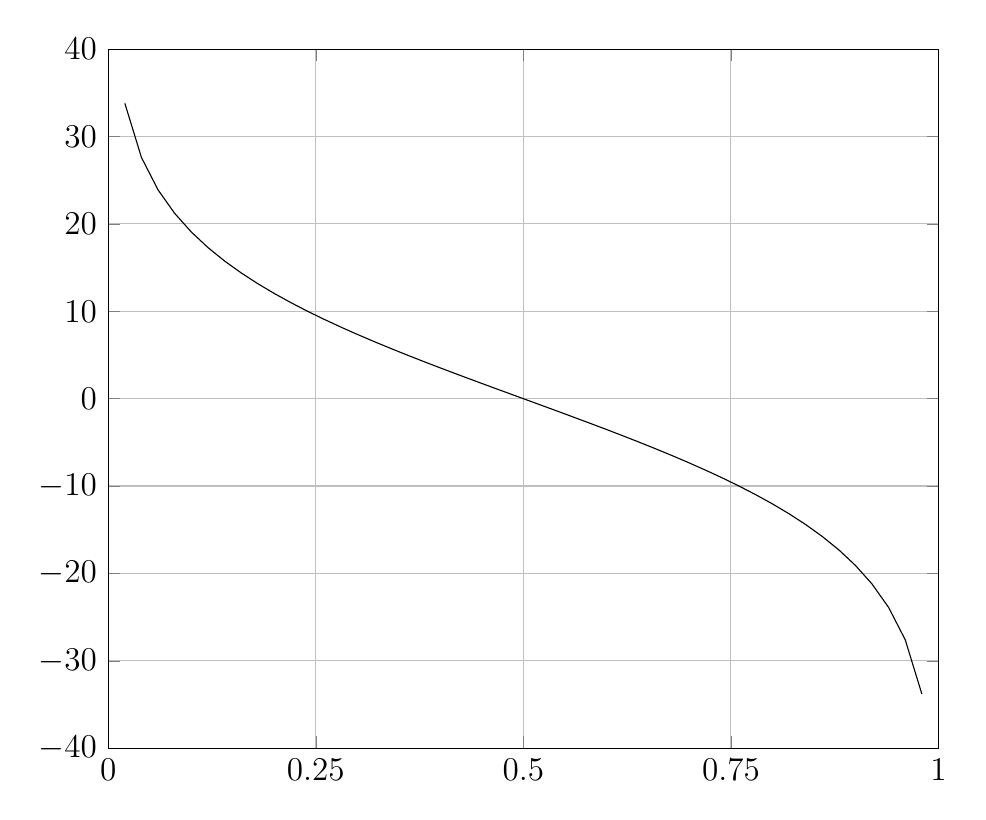
\begin{tikzpicture}
	        \begin{axis}[
                    width = \textwidth,
                    xmin=0, xmax=1,
                    ymin=-40, ymax=40,
                    xtick distance=0.25,
                    ytick distance=10,
                    grid=both
                ]
                \addplot[
                    domain=0:0.98,
                    samples=50,
                ]{20*log10((1-x)/x))};
	        \end{axis}
        \end{tikzpicture}
        \caption{$20\text{log}(\frac{1-x}{x})$}
        \label{fig:invamp-gain-a}
    \end{subfigure}
    \hspace*{\fill}
    \begin{subfigure}{0.5\textwidth}
        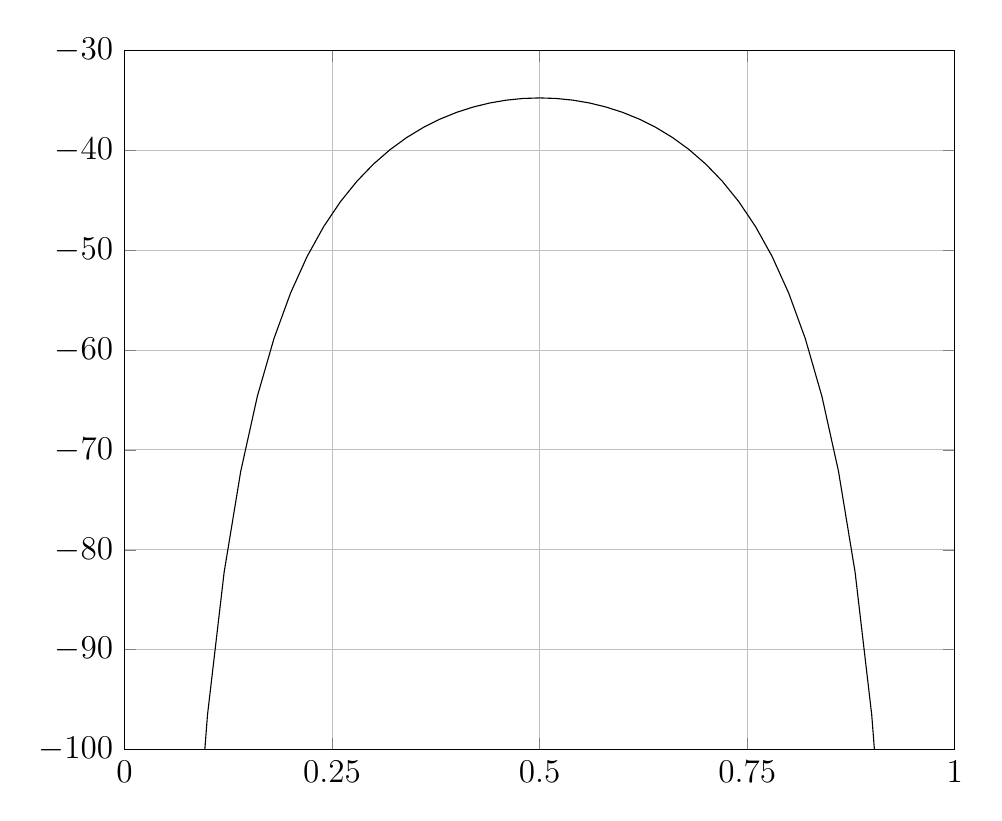
\begin{tikzpicture}
	        \begin{axis}[
                    width = \textwidth,
                    ymin=-100, ymax=-30,
                    xmin=0, xmax=1,
                    xtick distance=0.25,
                    ytick distance=10,
                    grid=both
                ]
                \addplot[
                    domain=0:0.98,
                    samples=50,
                ]{20/((x-1)*x*ln(10))};
	        \end{axis}
        \end{tikzpicture}
        \caption{$\frac{d}{dx}20\text{log}(\frac{1-x}{x})$}
        \label{fig:invamp-gain-b}
    \end{subfigure}
    \caption{Plot of the gain function and it's derivative}
    \label{fig:invamp-gain}
\end{figure}

\begin{figure}[H]
    \center
    \includesvg[
        width=\textwidth,
        height=0.3\textheight
    ]{media/opamps-invfilt}
    \caption{Active band pass filter}
    \label{fig:invfilt}
\end{figure}

Adding reactive components to an amplifier's circuitry is only natural, it
allows selective manipulation of the voltage gain with respect to the
frequency. Figure \ref{fig:invfilt} shows such an example, forming an active
high pass and low pass filter chain (or a band pass filter) if $C_1 > C_2$.
The voltage gain of this filter is described by the equation:

\begin{equation}
    A_v(j\omega) =
        \frac{-j\omega C_1 R_2}{(1+j\omega C_1 R_1)(1+j\omega C_2 R_2)}
\end{equation}

An intuitive understanding of this configuration's gain amplitude can be
formed: at low working frequencies, the capacitor C\sub{1} forms a high
impedance with R\sub{1}, while capacitor C\sub{2} is shunted by R\sub{2} and
forms a comparatively low impedance so the voltage gain is low. For a working
frequency $\frac{1}{C_1R_1} < f < \frac{1}{C_2R_2}$, capacitor C\sub{1} has low
reactance and most of the impedance will come from R\sub{1}, while capacitor
C\sub{2} will still be shunted by R\sub{2}, so the voltage gain will be ratio
of the resistors. For a larger working frequency, capacitor C\sub{2} will shunt
resistor R\sub{2} instead and the voltage gain will be decrease again. This can
be seen in figure \ref{fig:bandpass}, where the two cutoff frequencies are
200Hz and 2kHz and the ratio of the resistors is 1.

\begin{figure}[H]
    \center
    \begin{tikzpicture}
        \begin{semilogxaxis}[
                width=0.8\textwidth,
                grid=both
            ]
            \addplot table [col sep=comma] {media/bandpass.csv};
        \end{semilogxaxis}
    \end{tikzpicture}
    \caption{Example bandpass transfer function}
    \label{fig:bandpass}
\end{figure}


\subsection{Non-inverting amplifiers}

\begin{figure}[H]
    \center
    \includesvg[
        width=\textwidth,
        height=0.3\textheight
    ]{media/opamps-amp}
    \caption{Opamp non-inverting amplifier}
    \label{fig:noninvamp}
\end{figure}

The non-inverting amplifier, seen in figure \ref{fig:noninvamp}, has only one
function: it amplifies signals\cite{serban}. As opposed to the inverting amplifier, the
voltage gain has to be at least equal to 1, if not greater, as seen in the
equation:

\begin{equation}\label{eq:noninvamp}
    A_v = 1 + \frac{R_2}{R_1}
\end{equation}

Similarly to the inverting amplifier, inserting a potentiometer in the feedback
loop allows the voltage gain to be adjustable, and it will follow the equation:

\begin{equation}
    A_v = 1 + \frac{(1-p)+\frac{R_2}{R_p}}{p+\frac{R_1}{R_p}}
\end{equation}

\begin{figure}[H]
    \begin{subfigure}{0.5\textwidth}
        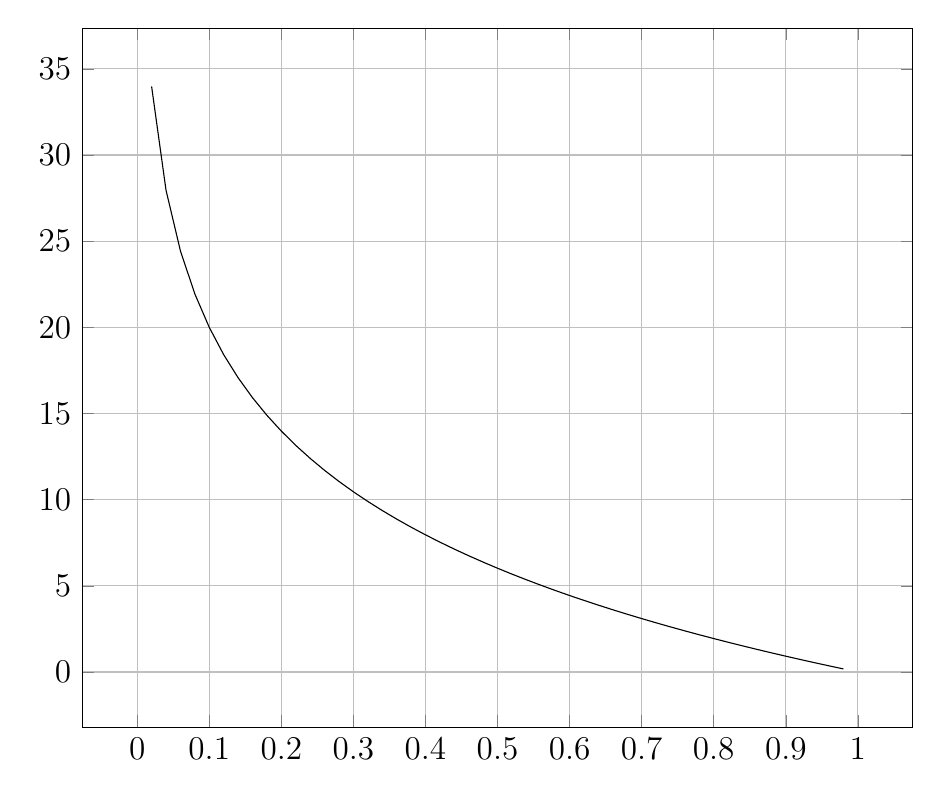
\begin{tikzpicture}
            \begin{axis}[
                    width = \textwidth,
                    grid=both
                ]
                \addplot[
                    domain=0:0.98,
                    samples=50
                ]{20*log10(1+(1-x)/x)};
            \end{axis}
        \end{tikzpicture}
        \caption{$\frac{d}{dx}20\text{log}(1+\frac{1-x}{x})$}
        \label{fig:noninvamp-gain-a}
    \end{subfigure}
    \hspace*{\fill}
    \begin{subfigure}{0.5\textwidth}
        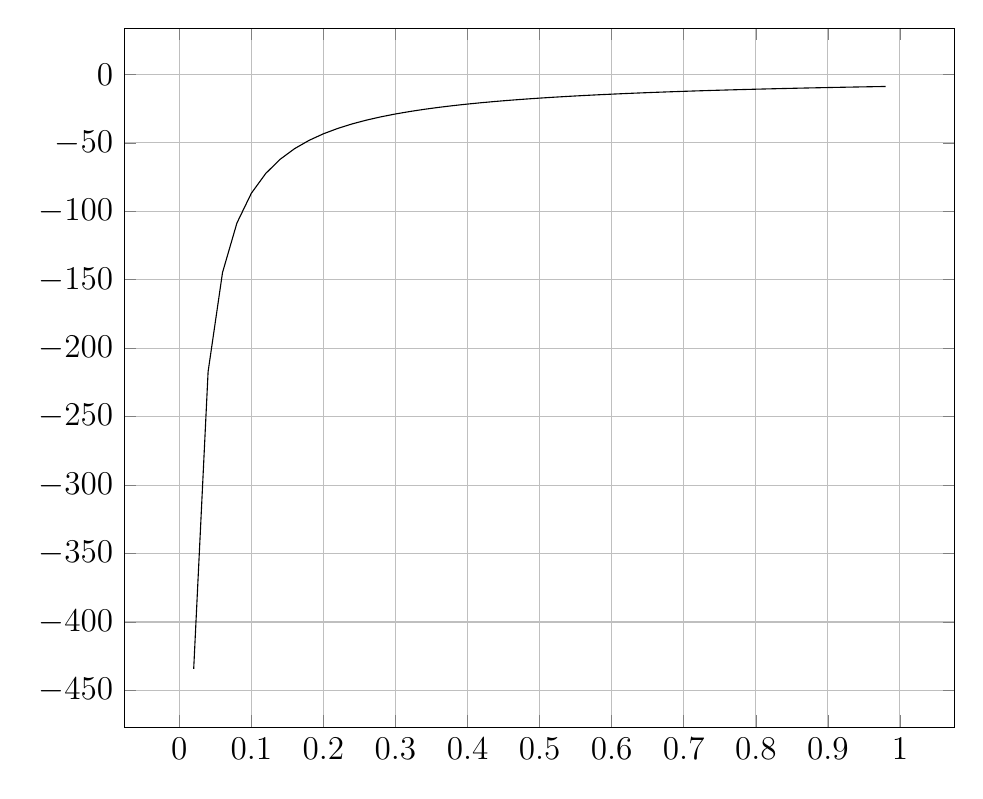
\begin{tikzpicture}
            \begin{axis}[
                    width = \textwidth,
                    grid=both
                ]
                \addplot[
                    domain=0:0.98,
                    samples=50
                ]{-20/x/ln(10)};
            \end{axis}
        \end{tikzpicture}
        \caption{$\frac{d}{dx}20\text{log}(1+\frac{1-x}{x})$}
        \label{fig:noninvamp-gain-b}
    \end{subfigure}
    \caption{Plot of the gain function and it's derivative}
    \label{fig:noninvamp-gain}
\end{figure}

Simplifying the equation and converting the result to dB yields the two graphs
seen in figure \ref{fig:noninvamp-gain}. The ratios $\frac{R_2}{R_p}$ and
$\frac{R_1}{R_p}$ will determine the maximum and minimum gain values of the
stage, as well as the linearity of the curve. However, in order to create a
more linear curve, the gain range has to be substantially reduced compared to
the inverting amplifier. A potentiometer with logarithmic taper would be
necessary to maintain both the range and the linearity.

\begin{figure}[H]
    \center
    \includesvg[
        width=\textwidth,
        height=0.3\textheight
    ]{media/opamps-noninvfilt}
    \caption{Noninverting bandpass filter}
    \label{fig:noninvfilt}
\end{figure}

Figure \ref{fig:noninvfilt} shows an example of a bandpass filter created with
a noninverting stage. In truth, these are two passive filters with the opamp
acting as a buffer between the two, and figure \ref{fig:bandpass} will be
representative of the transfer function of this configuration.

\begin{figure}[H]
    \begin{subfigure}{\textwidth}
    \center
    \includesvg[
        width=\textwidth,
        height=0.44\textheight
    ]{media/opamps-lowshelf}
    \caption{Low frequency shelf}
    \label{fig:lowshelf}
    \end{subfigure}
    \begin{subfigure}{\textwidth}
    \center
    \includesvg[
        width=\textwidth,
        height=0.44\textheight
    ]{media/opamps-highshelf}
    \caption{high frequency shelf}
    \label{fig:highshelf}
    \end{subfigure}
    \caption{Noninverting shelves}
\end{figure}

Figure \ref{fig:lowshelf} shows an active filter. Intuitively, the capacitor
will shunt the top resistor at high enough frequencies, which will bring the
gain of the stage to unity, while at low frequencies the top resistor will
shunt the capactior and the voltage gain can be calculated according to
the equation of the non-inverting amplifier \ref{eq:noninvamp}.
Similarly, for figure \ref{fig:highshelf}, but the
behaviour is now reversed: at low frequencies the impedance of the bottom side
of the feedback loop will be large and the gain will be unity, while at high
frequencies the capacitor can be considered a short and the gain will follow
the same equation\cite{negrescu}. Figures \ref{fig:lowshelf-freq} and \ref{fig:highshelf-freq}
show examples of the transfer function for shelf configurations.

\begin{figure}[H]
    \center
    \begin{tikzpicture}
        \begin{semilogxaxis}[
                width = 0.7\textwidth,
                grid=both
            ]
            \addplot table[
                col sep=comma
            ]{media/lowshelf.csv};
        \end{semilogxaxis}
    \end{tikzpicture}
    \caption{Example low shelf transfer function}
    \label{fig:lowshelf-freq}
\end{figure}

\begin{figure}[H]
    \center
    \begin{tikzpicture}
        \begin{semilogxaxis}[
                width = 0.7\textwidth,
                grid=both
            ]
            \addplot table[
                col sep=comma
            ]{media/highshelf.csv};
        \end{semilogxaxis}
    \end{tikzpicture}
    \caption{Example low shelf transfer function}
    \label{fig:highshelf-freq}
\end{figure}


\subsection{Summing amplifiers}

\begin{figure}[H]
    \center
    \includesvg[
        width=\textwidth,
        height=0.3\textheight
    ]{media/opamps-invsum}
    \caption{Opamp inverting summing amplifier}
    \label{fig:invsumamp}
\end{figure}

Figure \ref{fig:invsumamp} shows an inverting summing configuration. The output
voltage of this stage is given by the equation:

\begin{equation}
    v_\text{out} = -R_f (\frac{v_\text{1}}{R_1} +
                         \frac{v_\text{2}}{R_2} + ... +
                         \frac{v_\text{n}}{R_n})
\end{equation}

If $R_1 = R_2 = ... = R_n$ then the voltage gain for each input will be
identical and will have the same formula as in the case of the inverse
amplifier. The gain for this stage can be made adjustable, but the
potentiometer has to have two of the pins short circuited and has to be
connected between $R_f$ and the negative input of the opamp, such that the
formula becomes:

\begin{equation}
    v_\text{out} = -((1-p)R_p + R_f) (\frac{v_\text{1}}{R_1} +
                         \frac{v_\text{2}}{R_2} + ... +
                         \frac{v_\text{n}}{R_n})
\end{equation}

This solution is unpractical, however, as the function in dB can not be made
linear with respect to the position of the wiper, even if the potentiometer had
a logarithmic or inverse log taper and the voltage gain for a single input will
be extremely large as the wiper position approaches 0, regardless of the values
of the resistors. An alternative solution would be connecting the potentiometer
in a manner similar to that of the inverting amplifier, but it results in
unnecessarry attenuation at the inputs, an attenuation that will be larger as
more inputs are added tot the stage.

\begin{figure}[H]
    \center
    \includesvg[
        width=\textwidth,
        height=0.3\textheight
    ]{media/opamps-sumamp}
    \caption{Opamp non-inverting summing amplifier}
    \label{fig:sumamp}
\end{figure}

The non-inverting summing amplifier, seen in figure \ref{fig:sumamp}, has the
following formula for the output voltage:

\begin{equation}
    \begin{split}
    v_\text{out} = (1+\frac{R_t}{R_b})
        (&\frac{1}{1 + R_1 (R_2 || R_3 || ... || R_n)^{-1}} v_\text{1}
      \\+&\frac{1}{1 + R_2 (R_1 || R_3 || ... || R_n)^{-1}} v_\text{2}
  \\+...+&\frac{1}{1 + R_n (R_1 || R_2 || ... || R_{n-1})^{-1}} v_\text{n} )
    \end{split}
\end{equation}

If $R_1 = ... = R_n$ then the voltage gain for each input will be identical and
will have the formula of the non-inverting amplifier multiplied by $n^{-1}$.
This means that in order to obtian a specific gain value $A_v$ the top resistor
in the feedback loop (R\sub{t}) has to have a value of $(nA_v+1)R_b$ which
means that it grows linearly with the number of inputs, voltage gain, and the
value of the bottom resistor.
Making the voltage gain of this stage adjustable is done identically to the
non-inverting amplifier, and will bring the same problems.

The discussions regarding adjustable gain show that these configurations are
not very favorable towards having their gain modified. As such, they are easier
to implement as fixed gain stages then add variable gain stages separately.


%\subsection{Baxandall tone control}
%
%\begin{figure}[H]
%    \center
%    
\includegraphics[width=0.8\textwidth]{media/baxandall}
%    \caption
%    [
%        Two band Baxandall tone control
%    ]
%    {
%        Two band Baxandall tone control
%        \cite{Self2020}
%    }
%    \label{fig:baxandall-2}
%\end{figure}


%%%%%%%%%%%%%%%%%%%%%%%%%%%%%%%%%%%%%%%%%%%%%%%%%%%%%%%%%%%%%%%%%%%%%%%%%%%%%%%%
% --- MIXING CONSOLE ARCHITECTURE -------------------------------------------- %
%%%%%%%%%%%%%%%%%%%%%%%%%%%%%%%%%%%%%%%%%%%%%%%%%%%%%%%%%%%%%%%%%%%%%%%%%%%%%%%%
\newpage
\section{Typical architectures of a mixing console}

The mixing console is undoubtedly one of the most challenging areas of analog
audio design, as the relentless advance of digital media demands near-perfect
performance in every stage of the process, from performer to consumer. The cozy
assurance that music would pass through the quality bottleneck of analog tape
or vinyl disc now seems decidedly old-fashioned. The professional mixing
console poses numerous and varied technical problems, many of which are unique
to console design.

A mixing console must accommodate a large number of signals in a limited space
while ensuring that they remain strictly separated until the operator chooses
to mix them; crosstalk must be kept to an absolute minimum. Each input channel
may have several stages, any of which could introduce distortion and noise into
the signal. Even seemingly simple tasks like summing signals together can be
quite challenging in practical application.

Recording console quality requirements are much more demanding than those for
the most expensive hi-fi equipment. Once degradation is introduced at this
stage, it cannot be retrieved, making it essential to minimize noise and
distortion in the console. Two primary requirements of modern consoles are very
low noise and minimal distortion.

Since a comprehensive console must pass the audio through numerous circuit
stages, it is crucial to pay close attention to detail at each stage to prevent
a buildup of noise and distortion. One of the most critical trade-offs is the
impedance of the circuitry surrounding the opamp. If it is too high, Johnson
noise will increase, and if it is too low, the opamp will exhibit non-linearity
while struggling to drive it.

Mixing consoles always strike a balance between noise and headroom when it
comes to their internal signal levels. A higher level implies that the signal
is less affected by circuit noise but increases the likelihood of accidental
overload, and vice versa. The level chosen depends on the console's intended
use. If you are recording, you need to get it right only once, but you must do
so precisely with the best possible signal-to-noise ratio. Therefore, the
internal level is usually set relatively high, such as -2 dBu (615 mVrms),
which provides a headroom of about 22 dB. In broadcast work, you only have one
chance to get it right, and a slightly compromised signal-to-noise ratio is
preferable to an overload. This is especially true since FM or DAB channels
have limited noise performance anyway. In this case, the internal levels are
much lower. The advantage of an internal level of -2 dBu is that it allows the
signal to be doubled, as is done by most balanced output stages, to reach the
professional +4 dBu level directly.

Mixing consoles have multiple input channels that can be grouped together and
then summed into a stereo mix for the final result. Some small mixers do not
have groups and instead mix directly to stereo.

Consoles come in two primary formats, namely split, separate-group, or
European-style, and in-line arrangements. The former features input channels
arranged in one bank to the left of the master section, with the groups banked
to the right. On larger consoles, there might be an additional set of channels
to the right of the groups. On the other hand, in-line consoles have channels
and groups built into the same module, with a row of channel/group modules to
the left and right of a central master section. In-line consoles are more
compact and efficient in terms of electronic facilities, but they may be more
challenging to use due to their conceptual complexity.

\subsection{Split-mixing architecture}

\begin{figure}[H]
    
\includegraphics[width=\textwidth]{media/split-mixer}
    \caption
    [
        Block diagram of a split format mixer
    ]
    {
        Block diagram of a split format mixer
        \cite{Self2020}
    }
    \label{fig:split-mixer}
\end{figure}

The architecture of split mixing involves each channel having both a microphone
and line-level input, along with a wide-ranging gain control. After the signal
has been elevated to the standard internal level of the console, it undergoes
processing by the equalization section, which is regulated by the channel
fader's level. The signal is then routed to a group or pair of groups or
directly to the stereo L-R bus. The panoramic potentiometer, often known as a
panpot, sets the position of the channel signal in the overall stereo image.
The channel also has auxiliary send controls that feed the channel signal to
the auxiliary buses. Pre-fade sends, which are used for foldback and are taken
off before the fader, help musicians hear the sound they are producing.
Post-fade sends, which are used for adding effects such as reverberation and
are taken off after the fader, are dependent on the fader position. The final
feed from the channel to the buses is the pre-fade-listen (PFL), which, when
pressed, sends the pre-fade channel signal to the master module via the PFL
bus, replacing the normal stereo mix feed to the control-room monitor (CRM)
loudspeakers.

Either the group or the monitor modules incorporate both the group section and
one or two monitor sections. The group section comprises a summing amplifier
that collects all the signals sent to its group bus and passes them through a
fader and output amplifier to the outside world. During recording, this group
signal is sent to one track of the recording machine. The monitor sections
allow already recorded tracks to be played back to the stereo mix bus via a
level control and a panpot, permitting an early estimation of the final mix's
sound. One of the monitor sections is switchable between the group output and
the track return, allowing the monitor mix to be composed of both currently
recorded tracks and those previously laid down. Due to space constraints, the
monitor return sections usually have only basic EQ or none at all, but they
always have a pre-fade aux send for foldback purposes. A post-fade send is also
highly useful, as the rough monitor mix is more convincing when reverberation
is added appropriately, known as "wet" monitoring. The monitor sections often
include a PFL switch.

\subsection{In-line mixer architecture}

\begin{figure}[H]
    
\includegraphics[width=\textwidth]{media/inline-mixer}
    \caption
    [
        Block diagram of an in-line mixer
    ]
    {
        Block diagram of an in-line mixer
        \cite{Self2020}
    }
    \label{fig:inline-mixer}
\end{figure}

The architecture of in-line mixing now involves the integration of
channel/group/monitor modules to perform the functions of group/monitor
modules. The group summing amplifier is now part of the channel, and
its gain is controlled by a rotary bus trim control to prevent
overloading. This control is typically placed out of the way at the top
of the module. The group signal is sent to the recording machine, and
the track return signal is received through a balanced amplifier. A
track/group switch selects either the group or track return signal for
metering and monitoring purposes. This switch includes a monitor fader
and monitor panpot, which send the signal to the stereo mix bus to
create a monitor mix. The monitor fader is typically a shorter fader
located on the channel, rather than the longer channel fader at the
front of the console. In some cases, a rotary monitor fader may be
included.

There are two main strategies for the operation of an in-line module.
The first method, at mixdown, involves switching SW1 to select the
track return signal instead of the line input, which sends the signal
to the stereo mix bus through the full capabilities of the channel.
This approach may also allow the monitor path to be utilized as an
additional effects return, with the line input jack serving as the
input connector for this purpose. Alternatively, the entire EQ section
can be moved from the channel to the monitor path, which would require
the use of the short monitor fader for level adjustment. This setup is
not ideal when there is a long fader readily available. To address this
issue, a switch called "fader flip" is implemented, which swaps the
function of the two faders, enabling the use of the long fader at
mixdown. This second approach can be quite complex, as it involves
significant reconfiguration when switching from record to mixdown mode.
On more advanced consoles, this process is handled entirely by
electronic switching, with global control from the master section,
requiring only one switch to change the console mode. Despite its
complexity, this method has been widely used.


\subsection{The Channel Module (Split Format)}

\begin{figure}
    \center
    
\includegraphics[height=0.9\textheight]{media/channel_module}
    \caption
    [
        Block diagram of a typical channel module for a small mixer
    ]
    {
        Block diagram of a typical channel module for a small mixer
        \cite{Self2020}
    }
    \label{fig:channel_module}
\end{figure}

The channel module features an input stage that offers both
switchable balanced mic and line inputs. The mic input possesses an impedance
of 1-2 kΩ, which is suitable for a microphone capsule with a sensitivity of 200
Ω. If phantom power (+48 V) is necessary to power the microphone, it can be
independently switched on each channel. The line input features a bridging
impedance of at least 10 kΩ. The mic preamplifier boasts a wide range of gain,
from 0 to 70 dB, whereas the line input has a more restricted range, from +20
to -10 dB. The track return from the recording device is connected to the line
input through the normalling contact of the line jack socket. This
configuration enables mixdown with full channel facilities as soon as the
mic/line switch is set to "line," provided no jack is inserted into the line
input to disrupt the normalling contact.

After the input stage, a switchable
high-pass filter is commonly used (usually -3 dB at 100 Hz) to remove
low-frequency disturbances captured by the microphone. This filter typically
has a second or third order, providing a roll-off of 12 or 18 dB per octave,
respectively.

The tone-control section, commonly referred to as "EQ" or
equalization, typically includes one or more mid-band resonance controls and
standard shelving Baxandall-type high and low controls. On most mixers, the EQ
section can be switched out to allow for before/after comparisons.

The following component is the insert point in the signal path, which
can be set up in certain designs to come before the equalization and dynamics
section. This point allows external processing units to be connected through a
jack or a pair of jacks. When no external units are connected, the "normalling"
contacts on the jack socket enable the signal to pass through unaltered.

The pre-fade-listen switch routes the post-insert signal to the master module
and monitor speakers separately from all other controls. A PFL-detect bus then
instructs the master module to switch the studio monitoring speakers from the
typical stereo mix bus to the PFL bus. The channel ON switch follows in the
chain, which may be either a mechanical or electronic mute block. The PFL feed
is taken off before the ON switch, so the channel signal is
always accessible.

The channel level in the mix is controlled by a linear fader
with a post-fade amplifier that typically provides 10 dB of gain. The panpot
sets the stereo positioning, with odd group numbers being treated as left and
even numbers as right.

The channel shown has three auxiliary sends, which
represent an extra mixing system that operates independently of the main
groups. The number and configuration of these sends significantly affect the
overall versatility of the console. Each send control provides a feed to a
console-wide bus that is centrally summed and then sent out of the console.
Sends come in two main types: pre-fade sends that are taken from before the
main channel fader, and post-fade sends that take their feed from after the
fader, so the send level falls or rises according to the fader setting.

Pre-fade sends are widely employed for foldback, which entails providing the
artist with a feed of their performance through headphones. This is essential
if electronic manipulation is part of the creative process and vital if the
artist is adding additional material that must be synchronized with
pre-existing recordings. In the latter case, the existing tracks are played
back to the artist via the pre-fade sends on the monitor sections.

Post-fade sends, on the other hand, are used as effects sends, with their
source following the fader. This ensures that the effect will be faded down at
the same rate as the untreated signal, maintaining the same ratio. The total of
all feeds to a specific bus is sent to an external effects unit, and the output
of this is returned to the console. This enables multiple channels to share one
expensive device, such as a high-quality digital reverb, which is more suitable
than patching processors into the channel insert points for this type of
purpose.

There are often various auxiliary sends available on a mixing console, ranging
from one to twelve or more. In the example shown, Aux 1 is a dedicated
pre-fade send that is commonly used for foldback purposes, while Aux 3 is a
dedicated post-fade send that is commonly utilized for effects like reverb. Aux
2, on the other hand, can be adjusted to be either pre- or post-fade. During
the track laying process, foldback sends are most commonly used, while effect
sends are most in demand during mixdown. Therefore, it is common for some or
all of the sends on a channel to be switchable pre- or post-fade. On more
advanced consoles, it is possible to switch every auxiliary send between pre
and post to provide the greatest flexibility. In the past, this required
manually pressing a switch on every input module, which was time-consuming,
especially on a 64-input console. However, more recent designs have simplified
the process by allowing the pre/post selection for each auxiliary bus to be set
with a single master switch that controls the solid-state pre/post switching in
each module.


\subsection{Effect Return Modules}

When dealing with intricate mixdowns, it may be essential to incorporate
various effects back into the mix. Although it is often feasible to utilize
unused monitor sections or channel modules for this purpose, this method may
not always be adequate. In such cases, specialized "effects return" modules may
need to be installed. These modules are designed to occupy the same space as a
channel module and usually possess features that lie between channels and
monitor sections. Depending on the requirements, two or even four of these
modules may be installed. The returned effect, which is now in stereo, such as
the output of a digital reverb unit, is typically added to the stereo mix bus
via level and pan controls.


\subsection{The Group Module}

\begin{figure}[h]
    \center
    
\includegraphics[width=\textwidth]{media/group_module}
    \caption
    [
        Block diagram representing a common group module
    ]
    {
        Block diagram representing a common group module
        \cite{Self2020}
    }
    \label{fig:group-module}
\end{figure}

Each mix bus is equipped with a summing amplifier that combines the signal from
the individual tracks to produce a group signal, which is then sent to an
insert for external processing. This insert is often arranged for
ground-cancelling operation since the summing amplifier inherently phase
inverts the signal, which must be returned to the correct polarity by another
amplifier stage before it is sent to the outside world. This second stage can
be easily arranged to be ground-cancelling at minimal cost. The signal from the
insert return goes to the group fader, which is a linear fader with a post-fade
amplifier that provides 10 dB of gain. The signal then goes to an output
amplifier suitable for driving the recording device, possibly through long
cables. On all but the most basic designs, this output is balanced. The second
major function of a typical group module is to enable the creation of a monitor
mix, which allows new tracks to be synchronized with previously recorded tracks
at roughly the same levels as they will have in the final mix. This is
essential for ensuring that new material can be aligned with existing content.

The necessity of utilizing tape recording machines required the monitor
playback to be conducted by the record head, as the playback head was
physically relocated and would have resulted in a delayed signal. As a result,
the quality of the monitor mix was compromised, as the record head was designed
for recording rather than playback. However, with the advent of digital
recording technology, this issue has become obsolete. The monitor section
typically includes a balanced line input to prevent ground-loop problems with
the recorder, a switching mechanism between the group and recorder return,
which enables the track being recorded to be integrated into the monitor mix,
as well as level and panpot controls. Although EQ is not frequently installed
due to space constraints, aux sends for foldback and effects are standard, as
adding reverb to the monitor mix enhances its realism. A PFL switch for each
monitor section is typically provided.

In general, a small number of tracks are ordinarily recorded simultaneously,
which enables the use of more monitor sections than groups. For instance, a
four-group mixer can be effectively used with an eight-track recorder by
connecting Group 1 to Track 1 and Track 5, Group 2 to Track 2 and Track 6, and
so on. The choice of which track to record is typically made at the recorder.
To make the most of this arrangement, it is recommended that each group module
have one actual group section and two monitor sections, which is why there is
typically no room for basic equalization in the monitor sections.

\subsection{The Master Module}

\begin{figure}[H]
    \center
    
\includegraphics[width=0.9\textwidth]{media/auxmaster_module}
    \caption
    [
        Block diagram of a typical master module for a small mixer
    ]
    {
        Block diagram of a typical master module for a small mixer
        \cite{Self2020}
    }
    \label{fig:master_module}
\end{figure}

The Master Module is an indispensable element in the audio mixing process, as
it is responsible for integrating the stereo mix bus and offering the necessary
amplifiers and faders for precise management. This section also comprises a
post-amp, a balanced output stage, and a source-select switch, which enables
quality checks of the final recording. Moreover, the PFL switches are
incorporated into the master module, allowing for effortless monitoring and
level adjustments. The module also features aux send buses, which can be
managed through summing and level controls. Lastly, the master module contains
switches for altering global settings, such as group/recorder switching and
pre/post operation of auxes, making it a flexible and necessary component of
the mixing process.

\subsection{The In-Line Channel Module}

\begin{figure}[h!]
    \center
    
\includegraphics[height=0.9\textheight]{media/inline_channel_module}
    \caption
    [
        Channel/group/monitor module for
        an in-line recording console
    ]
    {
        Channel/group/monitor module for
        an in-line recording console
        \cite{Self2020}
    }
    \label{fig:inline_channel}
\end{figure}

The in-line channel module presented in figure \ref{fig:inline_channel}
uses the first approach to in-line operation. Rather than moving the EQ and
other facilities into the monitor path, the source of the channel path is
switched to the track return for entering mixdown mode.
The group fader is no longer visible, but the summing amplifier gain can
be adjusted using a rotary "bus trim" control. This control's primary function
is to prevent overload, and it is essential that it alters the gain of the
actual summing amplifier rather than relying on a low-gain summing amplifier
with a level control and post amplifier following it. The former option
provides better protection against clipping and superior noise performance at
low gain settings. The bus trim control is rarely adjusted, so it can be
conveniently placed out of the way at the top of the inline module. The group
signal from the summing amplifier is sent to the recording machine via a
balanced or ground-cancelling output stage to avoid ground loops with the
multi-track recorder. The track return typically comes back via a balanced
amplifier for the same reason. A Track-Return/Group switch selects either the
group or track return signal for metering and the monitor path. This path
consists of a monitor fader (the "short fader") and a monitor panpot, which
send the signal to the stereo mix bus to create a monitor mix. It is important
to note that every inline module will have a meter, but it is not common to
provide meters for every channel on a split console. A monitor PFL switch is
provided so that an individual track return or group can be easily listened to.

The process of connecting the track return to the channel line input through
normalling contacts on the line input jack is convenient and requires minimal
effort when switching to mixdown. As previously mentioned, in this type of
in-line configuration, the monitor path serves as a duplicate of the channel
fader and panpot, which are used to control the signal coming from the
multi-track recorder. Therefore, the monitor path can also be utilized as an
additional effects return, similar to split consoles. In this case, the line
input jack is typically used as the input connector, but an extra insert point
may be provided in the monitor path for external line signals. The auxiliary
send system in an in-line module is designed with maximum flexibility in mind.
In this example, switches SW3-SW8 allow the sends to be toggled to receive
signal either pre- or post-fade from either the channel or monitor path. During
recording, the effect sends can be switched to monitor post-fade, enabling wet
monitoring. There are numerous variations of the aux send available on larger
consoles, including six or eight sends and even a stereo aux send with its own
panpot.

\section{Physical considerations regarding PCBs and ICs}

PCBs are available in configurations of two layers, four layers, and so forth
in multiples of two. Odd-numbered PCB layers are not utilized because
four-layer and higher PCBs are constructed by combining two-layer PCBs, and
leaving a layer unused does not reduce costs.

The need for three-layer PCBs arose when flat mixers began to be built entirely
on a single large PCB, eliminating the use of screened-cable connections to and
from the faders, which are time-consuming and expensive to manufacture and
connect. For cost efficiency, all connections had to be integrated onto the
PCB, but a four-layer design was less practical due to its expense. Typically,
routing switches are positioned above the fader, necessitating that tracks to
the fader cross the mix buses on both the send and return paths. Consequently,
on a two-layer PCB, there was considerable capacitive crosstalk from the fader
connections to the mix buses.

\begin{figure}[H]
    \center
    
\includegraphics[width=\textwidth]{media/pcb-3layer}
    \caption{A three layer PCB example}
    \label{fig:pcb-3layer}
\end{figure}

Figure \ref{fig:pcb-3layer} shows a possible implementation of this concept.
The mixing buses were located on the bottom side of the two-layer PCB. The top
copper layer served as a ground plane, fully covering the mix bus area. On top
of this, two wire links provided the send and return paths to the fader. These
wire links can be installed much faster than twin screened-cable connections
and can even be auto-inserted. This setup is generally needed only where
signals cross the mix buses, as no other part of the system is as susceptible
to capacitive crosstalk.

With a four-layer board, critical tracks can be protected by placing them
between two ground plane layers, shielding them effectively. If this is not
feasible and conditions are particularly challenging, a screened cable between
two points on the PCB is an alternative, but costly in terms of
assembly time. In cases where components with large surface areas, like
electrolytics, are interacting, a vertical metal wall might be necessary,
though this also adds to the cost.

For the two halves of a dual opamp, the manufacturer’s specifications indicate
that internal crosstalk between them is very low. However, it's best to avoid
routing different channels through the same opamp, as this brings surrounding
components into close proximity, increasing the risk of capacitive crosstalk.

Electrical cable is frequently specified by its cross-sectional area and
current-carrying capacity, with the resistance per meter rarely mentioned.
However, this parameter is crucial for evaluating permissible voltage drops and
predicting crosstalk between two signals sharing a common ground conductor.
Given the resistivity of copper, the length of the cable and the area given in
catalogues, the resistance can be computed:
\[R=\frac{\text{resistivity} \cdot L}{\text{area}}\]

This provides the resistance of a segment of cable, allowing it to be easily
considered as part of a potential divider to calculate the voltage drop along
its length.

It is also beneficial to calculate the resistance of a PCB track for similar
reasons. This is somewhat more complex due to the variety of units used in PCB
technology, making it challenging to determine the cross-sectional area of the
track.

In the USA, the UK, and likely other places, a mix of metric and imperial units
is common on PCBs. Many essential components come in dual-in-line packages
based on an inch grid, resulting in track widths and lengths often measured in
thousandths of an inch, commonly called "thou" in the UK and "mil" in the USA.
Conversely, PCB dimensions and fixing-hole locations are usually metric,
aligning with the global standard in metal fabrication and mechanical CAD
(except in the United States).
Additionally, in the UK, copper thickness is quoted in ounces (the
weight of a square foot of copper foil), adding to the potential for
dimensional confusion.

Standard PCB copper foil, known as one-ounce copper, has a thickness of 1.4
thou (35 microns). Two-ounce copper is twice as thick, and its additional cost
is minimal, typically around 5\% of the total PCB cost, making it an easy way to
halve track resistance without altering a satisfactory layout. Four-ounce
copper is available but less common and more expensive. When heavier copper
than two-ounce is needed, it is standard to plate two-ounce copper up to
three-ounce, with an additional cost of around 10\% to 15\%.



%%%%%%%%%%%%%%%%%%%%%%%%%%%%%%%%%%%%%%%%%%%%%%%%%%%%%%%%%%%%%%%%%%%%%%%%%%%%%%%%
% --- IMPLEMENTATION --------------------------------------------------------- %
%%%%%%%%%%%%%%%%%%%%%%%%%%%%%%%%%%%%%%%%%%%%%%%%%%%%%%%%%%%%%%%%%%%%%%%%%%%%%%%%
\chapter{Design choices, schematics, simulations and physical implementation}

\begin{figure}[H]
    \center
    \includesvg[height=0.81\textheight]{media/Design}
    \caption{Hierarchical schematic of the implemented mixer}
    \label{fig:sch_root}
\end{figure}

The chosen architecture for the project is the split-mixer architecture, with
only channel modules and a master module. Since the project also implements the
functionality of an audio interface, groups and auxiliary inputs and outputs
have been omitted.

Figure \ref{fig:sch_root} shows the modules of the implemented mixer and how
they will be connected together.
The three channel inputs and the output are connected with consumer line lebel
unbalanced audio RCA jacks. All the modules are implemented on the same PCB
and, as such, are connected together with tracks.

The following design considerations will apply to all the modules described in
the following sections:
\begin{itemize}
    \item All opamp ICs presented are part of the LMV3xx family,
        either the LMV358 or  LMV324 which are dual opamps and quad opamps
        respectively.\cite{lmv3xx}
    \item The whole board will be powered from the USB connection, a maximum
        voltage of 5V and maximum current of 500mA. An LDO regulator is used to
        power all the circuits at 3.3V.
    \item The internal level used by the mixer was chosen to be -16dBV, lower
        than the line level. This is necessary to avoid clipping.
    \item The 3.3V supply of the opamps converts to an ideal maximum signal
        level of 1.17V\sub{RMS} or +1.36dBV. This translates into a headroom of
        17.36dB. All the stages in the modules were calibrated for a maximum
        gain of 10dB, giving a maximum implemented signal level of -6dBV, a
        level that is theoretically low enough to minimise the risk of
        clipping.
\end{itemize}

\section{The Channel Module}

\begin{figure}[H]
    \center
    \includesvg[width=\textwidth]{media/Design-PREAMP-EQ_L1}
    \caption{Hierarchical schematic of half of the stereo channel module}
    \label{fig:sch_channel}
\end{figure}

The implemented channel module seen in figure \ref{fig:sch_channel} consists of
an input stage and an EQ stage, interconnected with the stereo audio codec.

The input stage begins with a DC blocking capacitor (C19 in the figure)
connected to a voltage divider (R9 and R10) further connected to the input of
an inverting amplifier (U2A). The DC blocking capacitor and the voltage divider
add a DC component to the input signal, while the inverting amplifier presents
an adequate impedance for a line in connection and brings the signal level down
to.
The inverse phase shifting
introduced by the first opamp is then corrected by the second opamp (U2B) in
the stage, which also controls the gain of the signal through the potentiometer
(RV1). The output of this stage is then sent to the audio codec section.

The EQ stage receives its signals from the output of the audio codec.
It consists of three parallel integration and derivation opamp configurations
(U3A, B and C), each of them acting as a band pass filter, with bands 20Hz to
200Hz, 200Hz-2kHz, 2kHz-20kHz. The fourth opamp (U3C) is in an inverting summer
configuration, adding together the outputs of the three filters. Fader RV5 acts
as a volume control for the channel, before the mixing stage.

\begin{figure}[H]
    \center
    
\includegraphics[width=\textwidth]{media/sim_preamp-ac}
    \caption{Multi-step AC simulation of the input stage}
    \label{fig:sim_preamp-ac}
\end{figure}

Figure \ref{fig:sim_preamp-ac} shows the frequency response of the input stage
for different wiper positions on the potentiometer.
The 0dB reference in this graph is line level. The different plots have no
distinct curvature, meaning the audio signals pass through the circuit
unaltered except for amplitude, as intended.

\begin{figure}[H]
    \center
    
\includegraphics[width=\textwidth]{media/sim_preamp-in}
    \caption{Simulation of the input impedance of the input stage}
    \label{fig:sim_preamp-in}
\end{figure}

\begin{figure}[H]
    \center
    
\includegraphics[width=\textwidth]{media/sim_preamp-out}
    \caption{Simulation of the output impedance of the input stage}
    \label{fig:sim_preamp-out}
\end{figure}

Figures \ref{fig:sim_preamp-in} and \ref{fig:sim_preamp-out} show the
input and output impedances of the stage varying with the frequency.
Each curve corresponds to a different setting of the potentiometer.
Both graphs suggest that the impedances are within the specifications.

\begin{figure}[H]
    \center
    
\includegraphics[width=\textwidth]{media/sim_preamp-noise}
    \caption{Simulation of the noise spectrum in the preamp stage}
    \label{fig:sim_preamp-noise}
\end{figure}

Using the available noise analysis tools in SIMetrix, the power spectrum can
be obtained, seen in figure \ref{fig:sim_preamp-noise} and the total noise of
this stage can be computed and will be -103.46dBV.

\begin{figure}[H]
    \center
    
\includegraphics[width=\textwidth]{media/sim_eq-ac-low}
    \caption{Low frequencies boost/cut}
    \label{fig:sim_eq-low}
\end{figure}

\begin{figure}[H]
    \center
    
\includegraphics[width=\textwidth]{media/sim_eq-ac-mid}
    \caption{Mid frequencies boost/cut}
    \label{fig:sim_eq-mid}
\end{figure}

\begin{figure}[H]
    \center
    
\includegraphics[width=\textwidth]{media/sim_eq-ac-high}
    \caption{High frequencies boost/cut}
    \label{fig:sim_eq-high}
\end{figure}

Figures \ref{fig:sim_eq-low}, \ref{fig:sim_eq-mid} and \ref{fig:sim_eq-high}
show the frequency response of the EQ section for different frequency bands and
different potentiometer settings. Since the integration and derivation opamp
configuration is, in essence, a high-pass filter followed by a low-pass filter,
it's only natural that towards the ends of the spectrum the amplitude will
always be lower. The location of the poles and zeroes of the transfer functions
also shift with the potentiometer settings.

\begin{figure}[H]
    \center
    
\includegraphics[width=\textwidth]{media/sim_eq-in}
    \caption{Input impedance of the EQ stage}
    \label{fig:sim_eq-in}
\end{figure}

\begin{figure}[H]
    \center
    
\includegraphics[width=\textwidth]{media/sim_eq-out}
    \caption{Output impedance of the EQ stage}
    \label{fig:sim_eq-out}
\end{figure}

Figures \ref{fig:sim_eq-in} and \ref{fig:sim_eq-out} show the input and output
impedances of the EQ stage, varying with frequency. The input impedance is
lower than typical for line level inputs, but not such that it will
categorically cause overloading of the codec's output. The output impedance on
on the other hand (measured at the opamp output, before the fader) is more than
adequate to drive the following stage.

\begin{figure}[H]
    \center
    
\includegraphics[width=\textwidth]{media/sim_eq-noise}
    \caption{Simulation of the noise spectrum in the EQ stage}
    \label{fig:sim_eq-noise}
\end{figure}

Using the available noise analysis tools in SIMetrix, the power spectrum can
be obtained, seen in figure \ref{fig:sim_eq-noise} and the total noise of
this stage can be computed and will be -105.69dBV.


\section{The Master Module}

\begin{figure}[H]
    \center
    \includesvg[width=\textwidth]{media/Design-MASTER_L}
    \caption{Hierarchical schematic of half of the master module}
    \label{fig:sch_master}
\end{figure}

The master module presented in \ref{fig:sch_master}, similarly to the channel
modules, begins with DC blocking capacitors and resistive voltage dividers which
re-center the received signal on the necessary DC component. Then the inverting
summer (opamp U16A in the figure) adds together the three channels, and sends
the resulting signal through the fader acting as a volume control (RV16) and
further on, to a final opamp stage (U16B) which presents and adequate impedance
for a line out connection.

\begin{figure}[H]
    \center
    
\includegraphics[width=\textwidth]{media/sim_master-ac}
    \caption{AC simulation of the master stage}
    \label{fig:sim_master-ac}
\end{figure}

As with the preamplifier stage, the frequency response of the master module
needs to be as flat as possible, since it is only meant to sum the signals
coming from the three channels. Figure \ref{fig:sim_master-ac} shows the
frequency response of the stage for a single active input. If all inputs were
active, the resulting curve would show a gain of 3 or roughly 10dB
(the sum of the three AC voltage sources, one connected to each input, being
three times higher than the signal coming through a single channel).
In practical terms, this would be a reflection of three signals that occupy the
whole audio spectrum, raising the chance of clipping. This is slightly
unrealistic in a studio scenario:
Ideally, in a studio, each channel (representing different instruments or
voices) will occupy a different frequency band, the result being a signal that
occupies the whole spectrum. A channel outputting a signal that occupies the
whole spectrum would mean a song, or something similar, is playing
through that channel, something that is more likely to happen in a live
scenario, such as PA or radio broadcast, where accompanying music would be
played.

\begin{figure}[H]
    \center
    
\includegraphics[width=\textwidth]{media/sim_master-in}
    \caption{Simulation of the input impedance of the master stage}
    \label{fig:sim_master-in}
\end{figure}

\begin{figure}[H]
    \center
    
\includegraphics[width=\textwidth]{media/sim_master-out}
    \caption{Simulation of the output impedance of the master stage}
    \label{fig:sim_master-out}
\end{figure}

Figures \ref{fig:sim_master-in} and \ref{fig:sim_master-out} show the input and
output impedances of this stange. As in the case of the channel module, the
output impedance is within the specifications of line level output, and the
input impedance is more than adequate to be driven by the EQ stage that
precedes it.

\begin{figure}[H]
    \center
    
\includegraphics[width=\textwidth]{media/sim_master-noise}
    \caption{Simulation of the noise spectrum in the master module}
    \label{fig:sim_master-noise}
\end{figure}

Using the available noise analysis tools in SIMetrix, the power spectrum can
be obtained, seen in figure \ref{fig:sim_master-noise} and the total noise of
this stage can be computed and will be -106.61dBV.


\section{Audio Codec Section}

\begin{figure}[H]
    \center
    \includesvg[width=\textwidth]{media/Design-PCM1}
    \caption{Hierarchical schematic of the audio codec circuitry}
    \label{fig:sch_codec}
\end{figure}

This section is realised using the PCM2903C integrated circuit.
The PCM2903C is a single-chip USB audio codec designed for various audio
applications, including audio recording and playback devices.
It integrates USB transceiver functionality, stereo ADC, stereo DAC, and an
audio interface into a single device.

The USB audio interface is compliant with USB 2.0 full speed technology (a
maximum transfer rate of 12Mbps) and supports USB HID (Human Interface Device)
for audio controls.

The ADC and DAC both support 16-bit resolution and sampling rates of up to
48kHz. In terms of audio performance, the typical SNR values are 89dB for the
ADC and 96dB for the DAC and the dynamic ranges are 89dB and 93dB respectively.
Both the ADC and the DAC conform with
consumer line level signals, and present the necessary impedances.

In terms of power management, it is powered from single supply of 3.3V and
draws a current of 54mA during operation.
\cite{pcm}

\begin{figure}[H]
    \center
    
\includegraphics[width=\textwidth]{media/pcm-startup}
    \caption{Startup of the PCM2903C}
    \label{fig:pcm-startup}
\end{figure}

For the implementation, seen in figure \ref{fig:sch_codec} the power input pins
are all connected with decoupling
capacitors to filter low frequency power supply noise. The integrated circuit
features a crystal oscillator and requires an external crystal resonator
(Y1 in the schematic) in order to function. The data transmission is
handled by a differential pair, connected at pins 1 and 2 (D+ and D-) of the
device. Both pins are connected to decoupling capacitors and the D+ also
features a pullup resistor for correct functioning. Pin SEL1 triggers the
integrated circuit's reset procedure, preparing it for functioning, as seen
in figure \ref{fig:pcm-startup}, as such it is connected to an RC network to
delay the procedure until after the power is supplied to the circuit.
The analog audio pins all feature DC blocking capacitors to prevent any DC
components or noise from passing through to the ADC or out from the DAC.

\section{USB Hub Section}

\begin{figure}[H]
    \center
    \includesvg[width=0.8\textwidth]{media/Design-USB HUB}
    \caption{Hierarchical schematic of the USB hub circuitry}
    \label{fig:sch_usbhub}
\end{figure}

The TUSB2046 is a 4-port USB 1.1 hub controller that allows for the expansion
of a single USB port into four downstream ports. It is designed for embedded
systems and peripheral devices requiring multiple USB connections. The device
complies with the USB 1.1 standard and supports both full-speed (12 Mbps).

In terms of power management, the integrated circuit is powered from a single
supply of 3.3V and draws a maximum current of 40mA.
\cite{tusb}
All power pins are similarly connected with decoupling capacitors to filter
power supply noise, as seen in figure \ref{fig:sch_usbhub}.
This integrated circuit also features a crystal oscillator
that requires an external crystal resonator to function properly (Y4 in the
schematic). Since only three channels are implemented, only three of the
downstream data pins of this device are used, the last differential pair is
connected to ground with two resistors (pins 23 and 24). All the downstream
data pins are otherwise connected simliarly to the PCM2903C data pins, with
decoupling capacitors and pull down resistors. The upstream data pins again
follow the same pattern and are further connected to the mini USB type B port.
Pin 4 of this device acts as enable pin and is also connected to an RC network
that controls delays the startup of circuit.
In terms of transfer rate, since each codec produces 16-bit stereo samples and
48000 samples per second, the total necessary bandwidth is 9.2Mbps for
bidirectional communication, less than the available 12Mbps offered by the
integrated circuits. Furthermore, the total delay introduced by the digital
communication on the board is 4ms, 2 upstream transfers and 2 downstream
transfers, each of needing 1ms to be accomplished, as defined by the USB full
speed standard\cite{usb20}.

For power, the MCP1703A low dropout voltage regulator was used. It supplies the
whole board with 3.3V obtained from the 5V bus pin of the USB port. It supplies
a maximum current of 250mA, more than the 202mA necessary for the operation of
the codecs and the usb hub circuits, with enough room to power the analog
circuitry as well.

\section{PCB Layout}

\vfill
\begin{figure}[H]
    \center
    
\includegraphics[width=\textwidth]{media/PCB_front}
    \caption{Front view of the PCB}
    \label{fig:pcb_front}
\end{figure}
\vfill
\begin{figure}[H]
    \center
    
\includegraphics[width=\textwidth]{media/PCB_back}
    \caption{Back view of the PCB}
    \label{fig:pcb_back}
\end{figure}

The PCB reflects the split-mixer architecture, the three channels are placed to
the left of the master module, the total size is 200mm by 146.5mm.
It features ground planes on both copper layers,
screening most of the tracks from crosstalk.

The front layer features all the digital components on the board while to back
layer features most of the analog components, effectively isolating the two
return paths of the signals from each other, to minimise the noise.

The three cannel modules are also copies of each
other, and all operational amplifiers are process only a single side of the
stereo audio signals, minimising crosstalk between the stereo channels and
between the two sides of each individual channel.

Furthermore, the tracks are 1oz copper (35 microns thick) and their widths are
0.3mm for tracks carrying signals and 0.4mm for power supply tracks. This
results in a resistance of
$1.6\frac{\Omega}{\text{m}}$ for the signal tracks and
$1.2\frac{\Omega}{\text{m}}$ for the power supply tracks.
Given the dimensions of the board, the maximum length of any straight track
can't be more than 200mm, and the resistance of that track will be at most
0.32\textOmega for signal tracks. Given the fact that most input impedances
were designed to be in the magnitude of tens of kiloOhms, voltage mismatch
between stages as a result of track resistance will be minimal.

For the differential pairs between the digital components, care was taken such
that each pair is screened from others and that they cross as few of the
analog signal tracks as possible.

All passive components were placed as close as possible to the integrated
circuits on both sides of the board, the exception being the potentiometers and
the faders.

As of the 27th of June, the board was not completely assembled. Out of the 410
components, only around 150 were placed on the board, covering one channel
module with the associated codec section and the usb hub section. Figures
\ref{fig:statfront} and \ref{fig:statback} show the partial assembly of the
board.

\begin{figure}[h]
    \center
    
\includegraphics[width=\textwidth]{media/pcblicenta2}
    \caption{Assembly of the front side of the PCB}
    \label{fig:statfront}
\end{figure}

\begin{figure}[h]
    \center
    
\includegraphics[width=\textwidth]{media/pcblicenta1}
    \caption{Assembly of the back side of the PCB}
    \label{fig:statback}
\end{figure}





%%%%%%%%%%%%%%%%%%%%%%%%%%%%%%%%%%%%%%%%%%%%%%%%%%%%%%%%%%%%%%%%%%%%%%%%%%%%%%%%
% --- CONCLUSIONS ------------------------------------------------------------ %
%%%%%%%%%%%%%%%%%%%%%%%%%%%%%%%%%%%%%%%%%%%%%%%%%%%%%%%%%%%%%%%%%%%%%%%%%%%%%%%%
\chapter{Conclusions}

The first chapter represents a brief overview of audio equipment, both past and
present, with emphasis on the advantages and disadvantages of both analog and
digital audio processing techniques. The motivation of this thesis, the
structure and the specifications of the implemented equipment were also
presented.

The second chapter covered the theoretical aspects necessary for implementing
audio production equipment, emphasizing aspects about audio signals, noise
sources in audio circuitry, opamp and their configurations and audio mixer
architecture as well as the physical limitations that have to be taken into
account when taking the step from schematics to physical implementation.
Discussion of advantages and disadvantages of the configurations were also
introduced when warranted.
As such, this chapter elaborates on the parameters of audio
equipment, such as noise floor, headroom, dynamic range, input and output
impedances, on the parameters of the operational amplifiers which are used in
the circuitry, on their possible configurations and the viability of their uses
in audio equipment, on the two types of architectures (split mixing and
in-line) and the different modules that form an audio mixer (the two variations
of the channel modules, the master module, the effect return and group
modules), on the necessity of minimising channel crosstalk on the pcb and in
cables as well as methods of reducing it and the importance of track and cable
resistances.

The third chapter covers the design steps and physical implementation of the
mixer, covering the analog modules and the digital sections of the circuit.
The analog modules followed a simplified version of the split-mixing
architecture and they present adequate impedances at both the inputs and output
of the circuitry and have adequate values for noise floor, signal to noise
ratio, headroom and dynamic range, as seen in the simulation results. The
schematics for all sections were realised with the device electrical
characteristics and the manufacturer recommendations in mind. The PCB layout
was also realised considering all the effects listed in Chapter 2.

The following table shows the parameters of interest achieved in simulations
versus the specified requirements:

\begin{table}[H] \center
    \begin{tabular}{
            c c c
        }
        \hline\hline
        Parameter
        & Spec
        & Simulation\\
        \hline\hline
        Dynamic Range
        & 80dB
        & 101dB\\
        \hline
        Signal to Noise Ratio
        & 80dB
        & 84dB\\
        \hline
        Headroom
        & 16dB
        & 17dB\\
        \hline
        Input impedance
        & 10k\textOmega
        & 11k\textOmega\\
        \hline
        Output impedance
        & 600\textOmega
        & 350\textOmega\\
        \hline\hline
    \end{tabular}
    \caption{Performance parameters in simulation vs. spec}
    \label{table:parameters}
\end{table}

\newpage
\section{Further development}

Since the PCB is not fully assembled at the time of writing, the first
development would be finishing the assembly of the board, and measuring the
performance of the stages, in a manner similar to that used in the simulations.
Finishing the board assembly translates to placing the components for the
remaining two channel modules and the master module.
Measuring the performance of the device involves modifying the layout to allow
the connection of a Bode Analyzer to the board at multiple points. More
concretely, a 50\textOmega resistor needs to be added at every stage input, to
connect the AC disturbance source to it, pin headers need to be added at every
input and output and in between the stages to be able to measure the frequency
response.

Furthermore, several design choices in this project have yielded less than
ideal results, as seen in chapter 3.
In order to remedy that, some options for further development are available,
examples include:

\begin{itemize}
    \item Using Baxandall configurations for the EQ section, which
        have transfer functions that are symmetrical to the 0dB line when
        adjusting the potentiometers and also have more consistent frequency
        bands.
    \item Adding more input connectors, like XLR and TS/TRS Jack,
        for microphones or instruments, as well as the possibility to connect
        mono audio sources, both balanced and unbalanced, with corresponding
        preamplifier sections.
    \item Adding switches to bypass the audio codecs, if they are not needed,
        or to mute channels.
    \item Using a PCB with more than two layers to make routing easier.
    \item Using opamps with larger and differential supply voltages, to
        increase the headroom.
    \item Using a USB hub with a shorter transfer time, to reduce delays.
\end{itemize}


\printbibliography
\addcontentsline{toc}{chapter}{Bibliography}

\end{document}
